\chapter{Etude théorique du problème}
\section{Historique et présentation du problème.}
Le problème mathématique des tours de Hanoï a été inventé par Édouard Lucas. Il annonce que ce problème est dû à un de ses amis, N. Claus de Siam , prétendument professeur au collège de Li-Sou-Stian .

Sous le titre « Les brahmes tombent », Lucas relate que « N. Claus de Siam a vu, dans ses voyages pour la publication des écrits de l'illustre Fer-Fer-Tam-Tam, dans le grand temple de Bénarès, au-dessous du dôme qui marque le centre du monde, trois aiguilles de diamant, plantées dans une dalle d'airain, hautes d'une coudée et grosses comme le corps d'une abeille. Sur une de ces aiguilles, Dieu enfila au commencement des siècles, 64 disques d'or pur, le plus large reposant sur l'airain, et les autres, de plus en plus étroits, superposés jusqu'au sommet. C'est la tour sacrée du Brahmâ. Nuit et jour, les prêtres se succèdent sur les marches de l'autel, occupés à transporter la tour de la première aiguille sur la troisième, sans s'écarter des règles fixes que nous venons d'indiquer, et qui ont été imposées par Brahma. Quand tout sera fini, la tour et les brahmes tomberont, et ce sera la fin des mondes2 ! ».

Comme indiqué ci-dessous, \textbf{le probleme} est ce que un jeu à 64 disques requiert un minimum de 264-1 déplacements (soit 18 446 744 073 709 551 615 déplacements). En admettant qu'il faille une seconde pour déplacer un disque, ce qui fait 86 400 déplacements par jour, la fin du jeu aurait lieu au bout d'environ 213 000 milliards de jours, ce qui équivaut à peu près à 584,5 milliards d'années, soit 43 fois l'âge estimé de l'univers (13,7 milliards d'années selon certaines sources).


\section{Définition formelle du problème.}
Le but est de déplacer des disques de diamètres différents d'une tour de
« départ » vers une tour d'« arrivée » en passant par une tour « intermédiaire », et ceci
en un minimum de coups, tout en respectant les règles suivantes :\\
• on ne peut déplacer plus d'un disque à la fois ;\\
• on ne peut placer un disque que sur un autre disque plus grand que lui ou sur
un emplacement vide.\\
En suppose que cette dernière règle est également respectée dans la configuration
de départ.
Ce problème, peut devenir très vite complexe. En effet, pour n disques le nombre de
déplacements nécessaires est au minimum de 2^n − 1. 
\par
Le déplacement des disques nécessite donc deux fois plus de temps à chaque fois qu’un disque est ajouté à la tour initiale.

La résolution du problème des tours de Hanoï est très étudiée en algorithmique où elle
sert notamment à montrer que l'utilisation de la récursivité pour résoudre de gros
problèmes peut produire des codes à la fois logiques, puissants et concis.
Nous allons dans ce partie theorique proposer une solution récursive des tours de Hanoï, puis évaluer sa complexité.
\section{Présenter la modélisation de la solution (Structure de données de la solution).}
Le problème de tour de Hanoi peut être aisément modélisé avec un algorithme récursif. 
\par
\begin{function}[H]
    \Begin{
       
            \uIf{n > 0}{
                \textbf{Hanoi(n-1,D,I,A);}\\
                \textbf{Deplacer D vers A;}\\
                \textbf{Hanoi(n-1,I,A,D);}\\
            }
    }
    \caption{Hanoi(n : entier ,D: tour ,I : tour,A : tour)}
    
\end{function}
\par
Départ, intermédiaire et arrivée représentent les 3 tours.\\
N est le nombre de disques à déplacer. Le disque numéro n représente le plus grand disque se trouvant en bas de l’empilement dans la tour initiale.\\
Le principe de l’algorithme consiste à déplacer n-1 disques de « départ » vers « intermédiaire », puis le disque n de « départ » vers « arrivée » pour enfin mettre les n- 1 disques sur la tour « arrivée ». Le déplacement des n-1 se fait en plusieurs étapes à travers les appels récursifs de la procédure, jusqu’à ce qu’il ne reste qu’un disque à déplacer.\\
La structure de donnee qui serve notre problematique respectants les lois (First In Last Out , Une seule disque deplacer a la fois ( Depiler ) ) c'est bien la structure de donnee \textbf{La pile.} donc on peut representer nos tours avec des piles ou la sommets et le disque le plus petit a deplacer . 
\section{Présenter l’algorithme de résolution avec calcul détaillé de sa complexité théorique.}
\subsection{L'Algorithme de résolution :}
La resolution de tel probleme consiste a utiliser une variable
\textbf{n}:  qui va representer le nombre des disques , \textbf{3 piles A , D , I} qui vas \textbf{respectivement} representer les pillets d'arrivee , depart et intermediare . \\ 
Pour déplacer une tour de n disques de D vers A, on effectue ces trois étapes : \\
- déplacer la tour des n-1 premiers disques de D vers I (étape qui nécessite xn-1 déplacements, d’où la récurrence) ;\\
- déplacer le plus grand disque de D vers A (un déplacement supplémentaire) ;\\
- déplacer la tour des n-1 premiers disques de I vers A (à nouveau xn-1 déplacements).\\
Nous pouvons le représenter via le pseudo code suivant :
\par
\begin{function}[H]
    \Begin{
       
            \uIf{n > 0}{
                \textbf{Hanoi(n-1,D,I,A);}\\
                \textbf{Empiler(A,Depiler(D));}\\
                \textbf{Hanoi(n-1,I,A,D);}\\
            }
    }
    \caption{Hanoi(n : entier ,D: pile ,I : pile,A : pile)}
\end{function}
\\
\subsection{Calcul de complexite temporel recursive}
Soit T le nombre d'instructions de l'algorithme Hanoi (ci-dessus),  \\
on a 2 appels recursive a n-1 disques et une instruction pour le deplacement Empiler(A,Depiler(D)) qui a 2 operations Empiler la pile A et depiler de D. On suppose que le temps d'empiler/ depiler est le même et on le note f1. \\
Donc T(n)=2T(n-1)+2f1\\
on a : \\
T(0)=f2 , f2 constante \\
T(1)=2f2+ 2f1\\
T(2) =2T(1)+ 2f1 = 4f2 + 6 f1 \\
T(3) =2T(2)+ 2f1 =  8f2 + 14f1 \\
\par
la coefficient de f2 : 2^n  \\ 
\par
la coefficient de f1 : 2*2^n - 2 \\
\par
et donc T(n) = 2^nf2 + (2*2^n -2)f1 \\
\par
On conclut là aussi que l'Algorithme de problème des « tours de Hanoi » a une complexité temporelle exponentielle.\\

En conséquence, la complexité temporelle O(n) de l'algorithme Hanoi est: \\

  \[ 
\left\{
\begin{array}{r c l}
T(n)= T(n) = 2^nf2 + (2*2^n -2)f1 \quad \quad \quad \quad \quad notation-exacte\\
T(n)=O(n)= O(2^n)\quad \quad \quad notation-asymptotique
\end{array}
\right.
\]
\\
\subsection{Calcul de complexite spatiale recursive}
Soit T le nombre d'instructions de l'algorithme Hanoi (ci-dessus),  \\
on a 2 appels recursive a n-1 disques la deuxieme se lance apres qu'on finit la premiere et donc on peut utiliser l'espace d'appel recursive 1 pour faire le traitement de la deuxieme , on a 3 piles ou la somme de contenu de toutes les piles ne depasse pas le nombre de disque n ( en total on a n disque soit initialement dans le disque de depart ou bien difusee entre les 3 disque )  \\
Donc T(n)=T(n-1)+n\\
on a : \\
T(0)=k , k est constant ( peut etre 0, NIL ) \\
T(1)=k+1\\
T(2) =k+2 \\
T(n)= k+ n  ; d'ou la complexite spatiale est de O(n).

\subsection{l'Algorithme de resolution Iterative}
la solution itérative de tour hanoi qui on a implémenté ce un result de un remarque dans le pattern des movements des disc fait par l"algorithm recursive\\
\{\\
-  start -> end ( ou end -> start)\\
-  start -> inter (ou inter -> start)\\
-  inter -> end (ou end -> inter)\\
\}repete jusqu a le nomber des movements (deplacement) des disc est 2^N-1 
\\
\par
\begin{function}[H]
    \Begin{
        
                \uIf{pilevide(to)}{
                \textbf{empiler(to,depiler(from));}\\
                } 
                \ElseIf{pilevide(from)}{
                \textbf{empiler(from,depiler(to));}\\
                
                 }\ElseIf{tetepile(from) > tetepile(to)}{
                \textbf{empiler(from,depiler(to));}\\
                }\Else{
              \textbf{empiler(to,depiler(from));}\\
                }
            
    }
    \caption{move(from : pile,to : pile)}
\end{function}
\begin{function}[H]
\textbf{Variables :}\\
    numOfMoves: entier;\\
    \Begin{
        $numOfMoves\leftarrow pow(2,n)-1$\;
            \If{n mod 2 != 0}{
            \For{$i \leftarrow 1$ \KwTo numOfMoves}{
                \uIf{n mod 3 == 1}{
                \textbf{move(start,end);}\\
                } 
                \ElseIf{n mod 3 == 2}{
                \textbf{move(start,inter);}\\
                
                 }\ElseIf{n mod 3 == 0}{
                \textbf{move(inter,end);}\\
                }                
            }
            }\Else {
                \For{$i \leftarrow 0$ \KwTo numOfMoves-1}{
                \uIf{n mod 3 == 1}{
                \textbf{move(start,end);}\\
                } 
                \ElseIf{n mod 3 == 2}{
                \textbf{move(end,inter);}\\
                
                 }\ElseIf{n mod 3 == 0}{
                \textbf{move(inter,start);}\\
                }    
            }}
    }
    \caption{HanoiIter(n : entier ,start: pile ,end : pile,inter : pile)}
\end{function}
\section{Présenter l’algorithme de vérification avec pseudo-code et calcul détaillé de sa complexité théorique.}
\subsection{L'Algorithme de vérification :}
L’algorithme de vérification consiste à vérifier la règle suivante : "le disque déplacé ne doit jamais être placé au-dessus d’un disque plus petit que lui".  
L’algorithme fonctionne suivant les étapes suivantes :
\begin{itemize}
\item On compare l’élément qui situe à l’indice i de la pile et son successeur i+1.
\item Si le p.array[i]>p.array[i+1] alors l’algorithme retourne faux
\item  Si on atteint la taille de la pile l’algorithme retourne vrai
\item Sinon on avance dans la pile et on répète l’étape 1
\end{itemize}
	

\par
\\
\begin{function}[H]
\textbf{Variables :}\\
    i: entier\;
    \Begin{
       
            \If{(p.sommet=-1)}{ 
                \textbf{return true;}\\
            }
            \ELSE{ \For{$i \leftarrow 1$ \KwTo p.sommet}{
            \If{pile.array[i]<pile.array[i+1]}{
              \textbf{return false;}
            }
            \textbf{return true;}
            }}
            \ENDIF
           
    }
    \caption{Verification(p : pile)}
\end{function}
\subsection{Complexité théorique}
La complexité  de l'algorithme de verification  est egale a la taille de la pile ça vaut dire le nombre de disques empilés (n) dans l'etat finale  d'ou la complexité est linéaire O(n)

\section{Présentation d'une instance du problème avec sa solution (un exemple).}
\\
Le jeu des tours de Hanoï est constitué de trois piquets, placés verticalement, et de n disques de taille décroissante. Les n disques sont initialement placés par taille décroissante autour du piquet le plus gauche. Le but du jeu  consiste donc à déplacer les disques jusqu’à parvenir à la situation finale dans laquelle tous les disques se retrouvent autour du piquet le plus droit par ordre de taille décroissante. 
\par
Les figures suivante représentent le déroulement de ce jeu ou le nombre de disque est égale à 4 (le nombre de déplacements 2^ 4 -1).
\par
\begin{figure}[H]
    \centering
        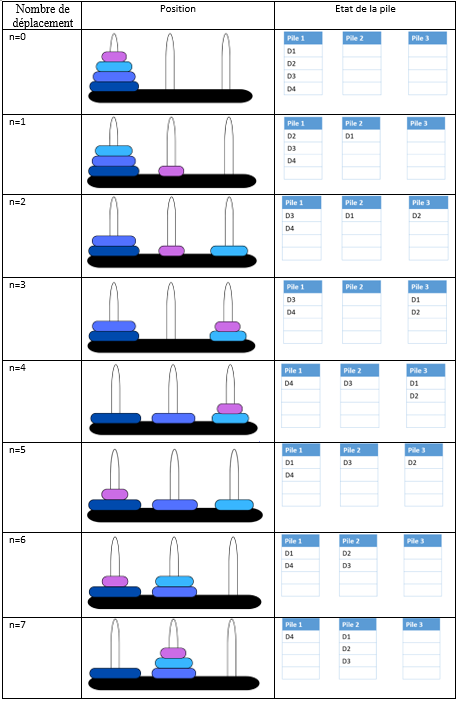
\includegraphics[scale=0.9]{ressources/deroulement1.png}
        
    \label{fig:derouelement1}
\end{figure}
\begin{figure}[H]
    \centering
        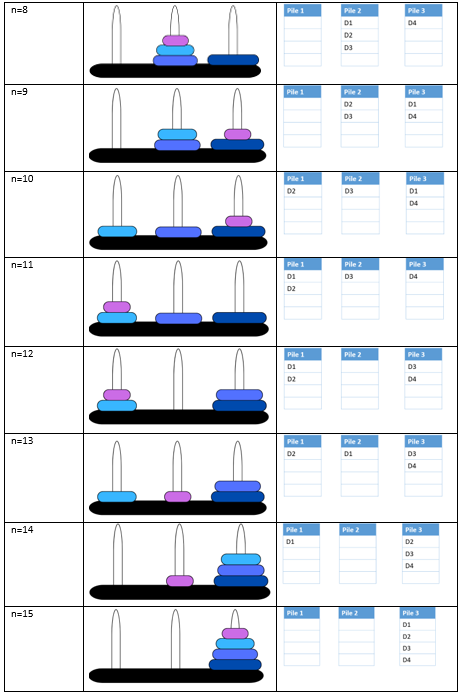
\includegraphics[scale=0.9]{ressources/deroulement2.png}
        
    \label{fig:derouelement2}
\end{figure}

